\subsection{Theory Exercises}

\subsubsection*{Bishop 11.3}

\subsection{Programming Exercise}

\subsection{Pyro}

The code is shown in~\cref{sec:week3:code:pyro}.
The plot of the GMM samples is shown in~\cref{fig:week3:pyro:gmm-samples}.
The plots of the densities $p(x_2 | x_1 = 2)$ and $p(x_2 | x_1 = 3)$
are shown in~\cref{fig:week3:pyro:cond-pdf}.

\begin{figure}[htbp]
  \centering
  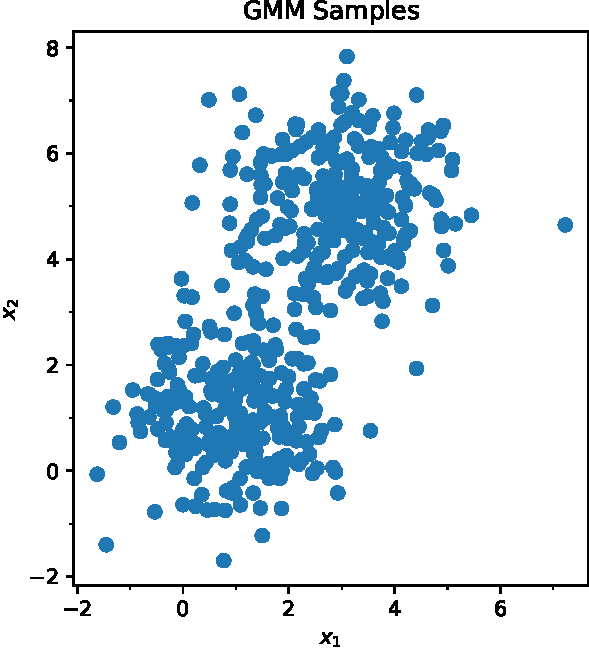
\includegraphics[width=0.5\textwidth]{./figures/gmm_samples.pdf}
  \caption{Scatter plot of 500 samples of the GMM.}
  \label{fig:week3:pyro:gmm-samples}
\end{figure}

\begin{figure}[htbp]
  \centering
  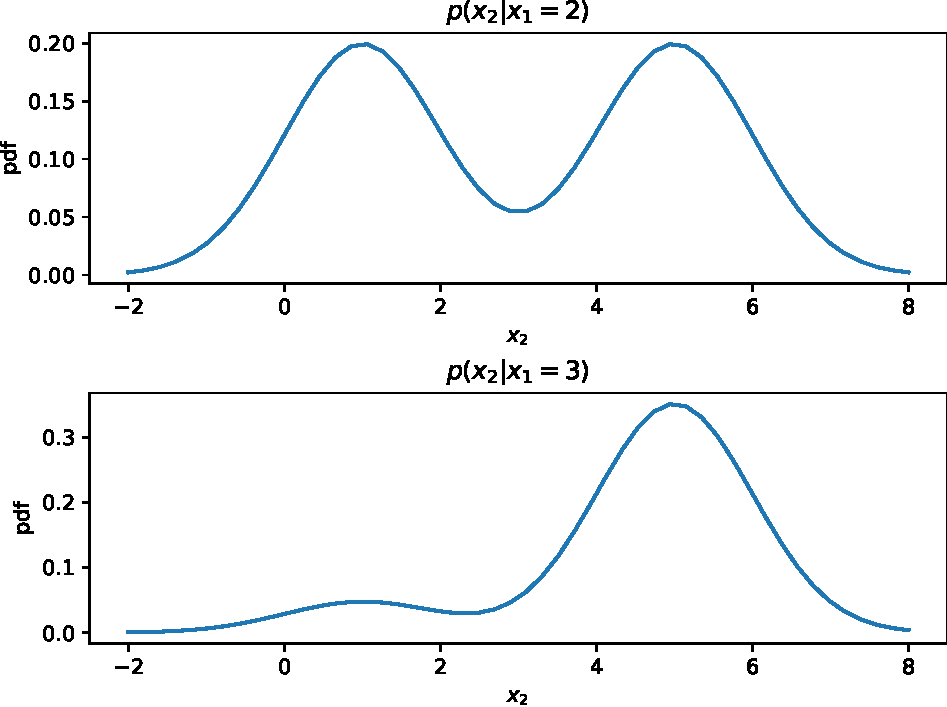
\includegraphics[width=0.7\textwidth]{./figures/cond_pdf.pdf}
  \caption{
    PDF of conditionals on $x_1$ of the GMM.
  }
  \label{fig:week3:pyro:cond-pdf}
\end{figure}
